\documentclass[a4paper]{article}

\usepackage[utf8]{inputenc}
\usepackage[T1]{fontenc}
\usepackage{textcomp}
\usepackage[english]{babel}
\usepackage{amsmath, amssymb}


%figure support
\usepackage{import}
\usepackage{xifthen}
\pdfminorversion=7
\usepackage{pdfpages}
\usepackage{transparent}
\newcommand{\incfig}[1]{%
	\def\svgwidth{\columnwidth}
	\import{./figures/}{#1.pdf_tex}
}
\graphicspath{ {./figures/} }
\pdfsuppresswarningpagegroup=1

\begin{document}
	\title{CIS4362.01 Homework 4 Due 12/6/19}
	\author{Brandon Thompson 5517}
	\maketitle

	\begin{enumerate}
		\item Draw the schematic view of all MAC and Encryption combinations which are
			implemented by programmers for providing authenticated encryption.
			Which combination always provides authenticated encryption?
			
			\begin{figure}[ht!]
				\centering
				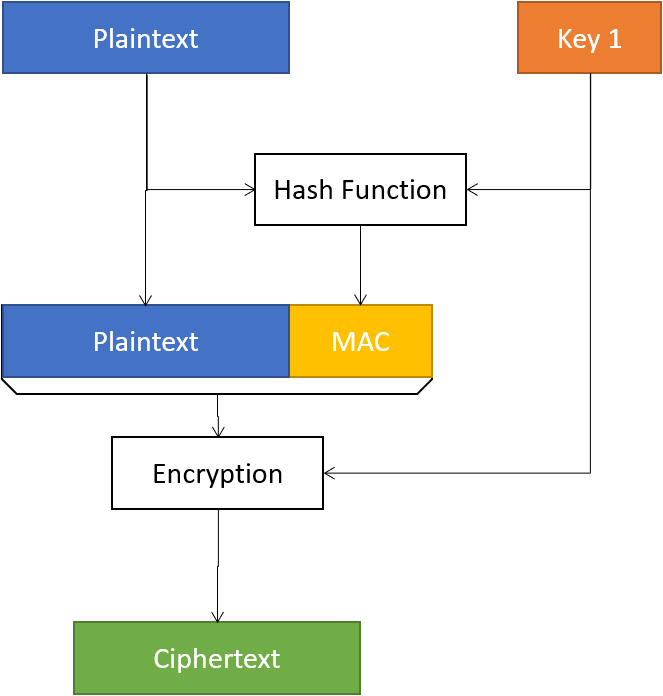
\includegraphics[width=0.8\textwidth]{mac_then_encrypt}
				\caption{Mac-then-encrypt (SSL).}
				\label{fig:mac_then_encrypt}
			\end{figure}

			\begin{figure}[ht!]
				\centering
				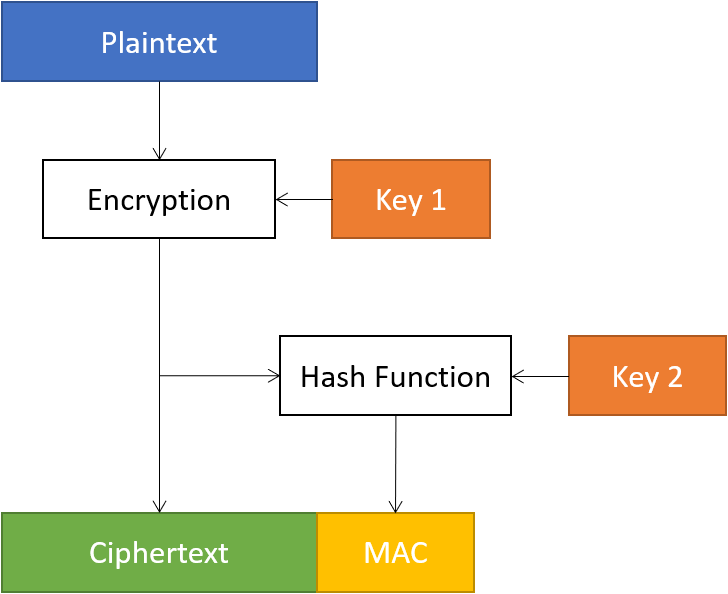
\includegraphics[width=0.8\textwidth]{encrypt_then_mac}
				\caption{Encrypt-then-mac (IPsec). Always provides authenticated encryption.}
				\label{fig:encrypt_then_mac}
			\end{figure}

			\begin{figure}[ht!]
				\centering
				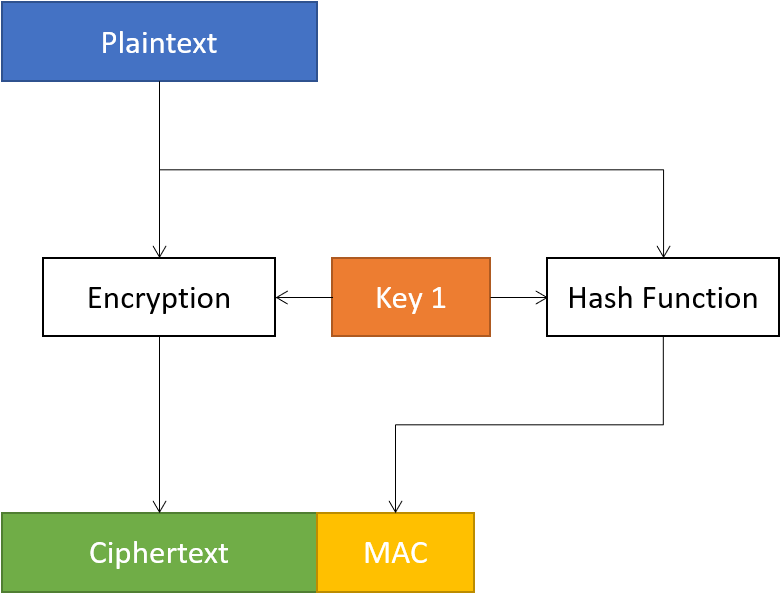
\includegraphics[width=0.8\textwidth]{encrypt_and_mac}
				\caption{Encrypt-and-mac (SSH).}
				\label{fig:encrypt_and_mac}
			\end{figure}
			\clearpage
		\item How a key be generated using Trusted 3rd Party (TTP) to enable a secure
			communication between two parties that have not exchanged their keys?
			Please draw the schematic and explain the way that this method works.
			\begin{figure}[ht!]
				\centering
				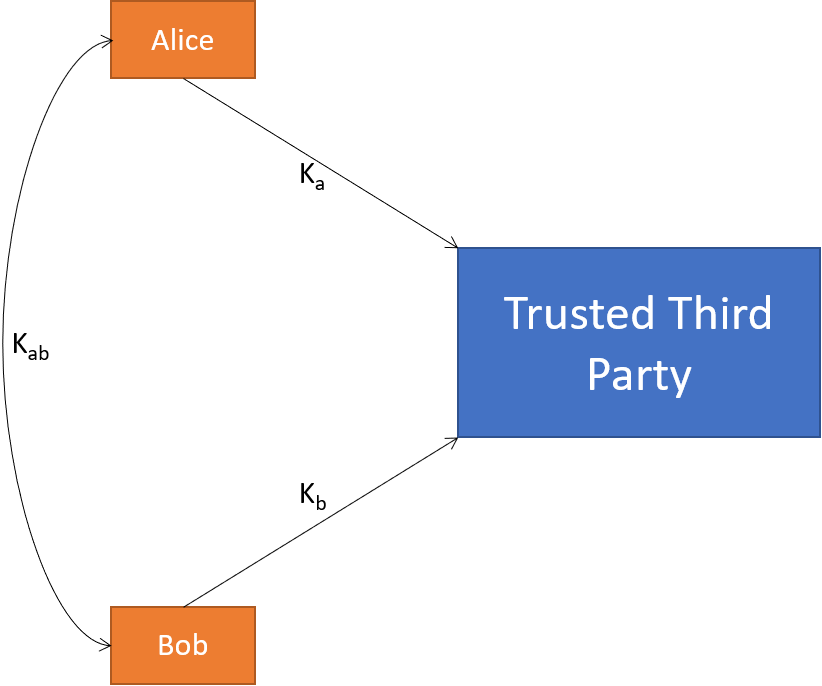
\includegraphics[width=0.8\textwidth]{trusted_third_party}
				\caption{Schematic drawing of trusted third party.}
				\label{fig:trusted_third_party}
			\end{figure}
			
			Trusted third party takes the keys of individuals and when notified that
			two users want to communicate, generates a random key $K_{ab}$ and encrypts
			and sends it to the users after encrypting it with their personal keys.
			Now the two users have a shared key and can communicate themselves.
		
		\item What are the drawbacks of using TTP in the real world? (list two drawbacks)
			\begin{itemize}
				\item TTP only secure against eavesdropping.
				\item TTP insecure against replay attacks.
				\item TTP is needed for all key exchanges (Kerberos), if compromised
					attacker has access to all keys.
				\item Can be targeted by denial of service (DOS) attack to stop new
					communications.
			\end{itemize}
		\clearpage
		\item What is the runtime of each of the following participants in Merkle puzzle?\\
			Alice: $O\left( n \right) $\\
			Bob: $O\left( n \right) $\\
			Eavesdropper: $O\left( n^{2} \right) $\\

		\item Draw the schematic view and explain a scenario in which Alice and Bob exchange
			the keys using Diffie-Hellman protocol.
			\begin{figure}[ht!]
				\centering
				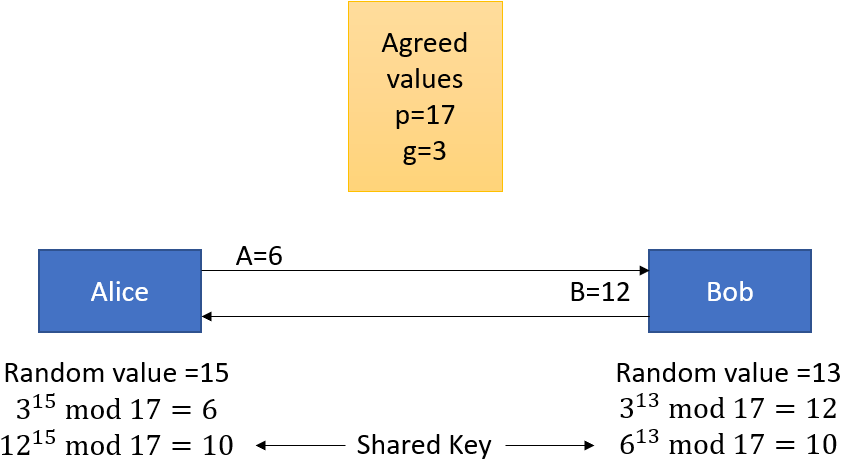
\includegraphics[width=0.8\textwidth]{diffie_hellman}
				\caption{Schematic view of Diffie-Hellman protocol.}
				\label{fig:diffie_helman}
			\end{figure}

			Bob and Alice agree publicly on a prime number $p$ and an integer
			$g \in \left\{ 1,\ldots,p \right\}$ Alice chooses a random value
			$a \in \left\{ 1,\ldots,p-1 \right\}$ and calculates $g^{a} \text{ mod } p = A$ and sends
			this to Bob. Bob also picks a random value $b \in \left\{ 1,\ldots,p-1 \right\}$
			and calculates $g^{b} \text{ mod } p = B$ and sends this to Alice.
			Now Alice would calculate $B^{a} \text{ mod } p$ to get the shared key.
			Bob would calculate $A^{b} \text{ mod } p$ to get the shared key.\\
			\\
			The final calculations are the same because:
			\begin{align*}
				B^a \text{ mod }p = g^{b^a} \text{ mod } p &= g^{ba} \text{ mod } p\\
				A^b \text{ mod }p = g^{a^b} \text{ mod } p &= g^{ab} \text{ mod } p
			\end{align*}
			which are equivalent.
	\end{enumerate}

\end{document}
